\chapter{Aufbau der Dateiformate}
\begin{figure}[ht]
	\centering
	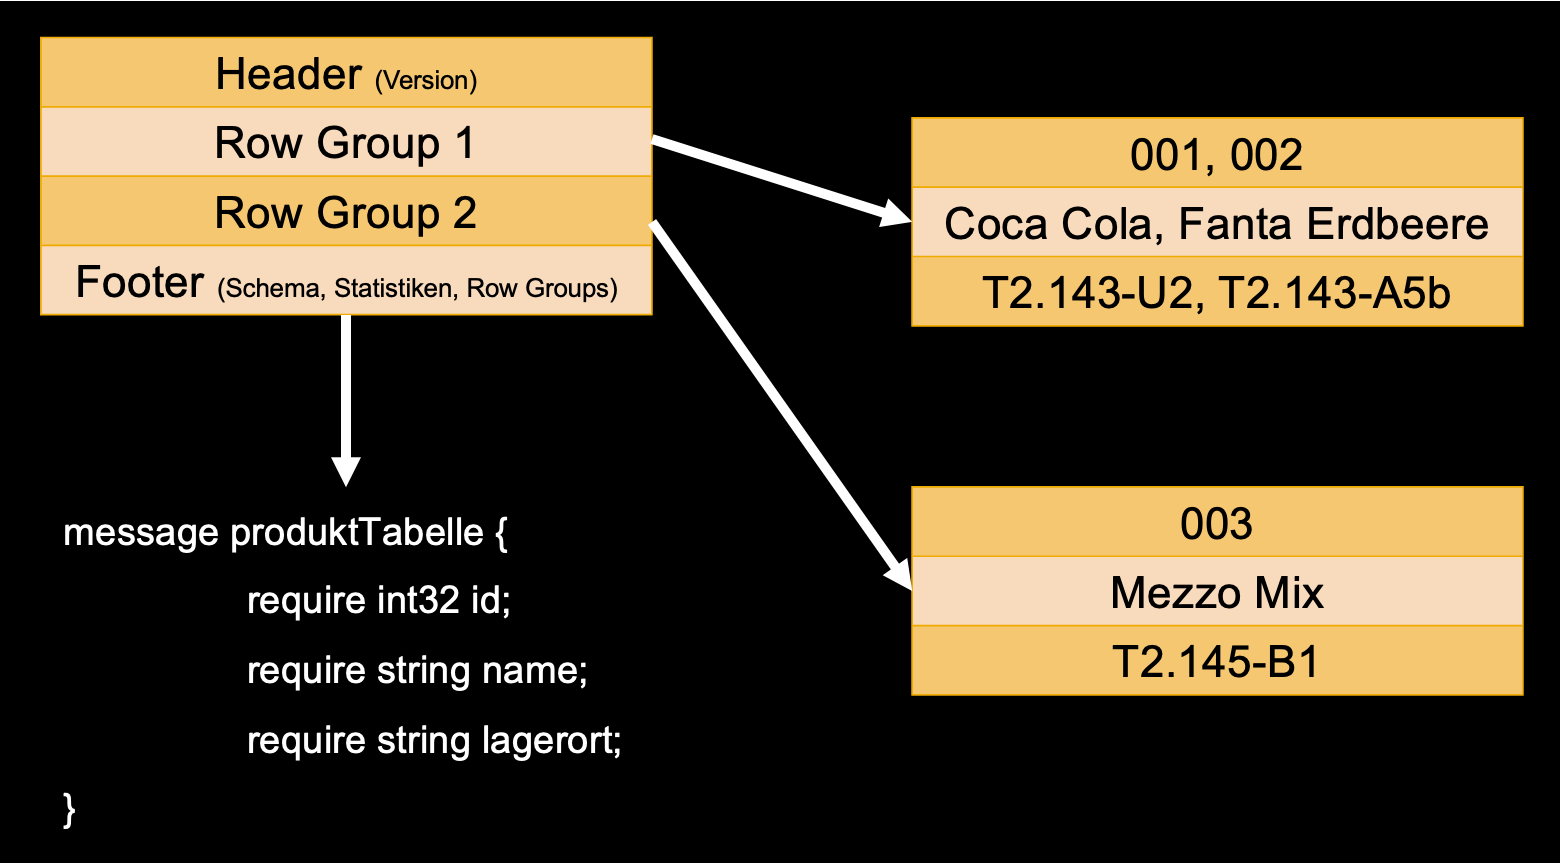
\includegraphics[width=1\textwidth]{Bilder/Parquet.png} 
	\caption{Aufbau von Parquet}
	\label{fig:Parquet}
\end{figure}
\clearpage
\begin{figure}[ht]
	\centering
	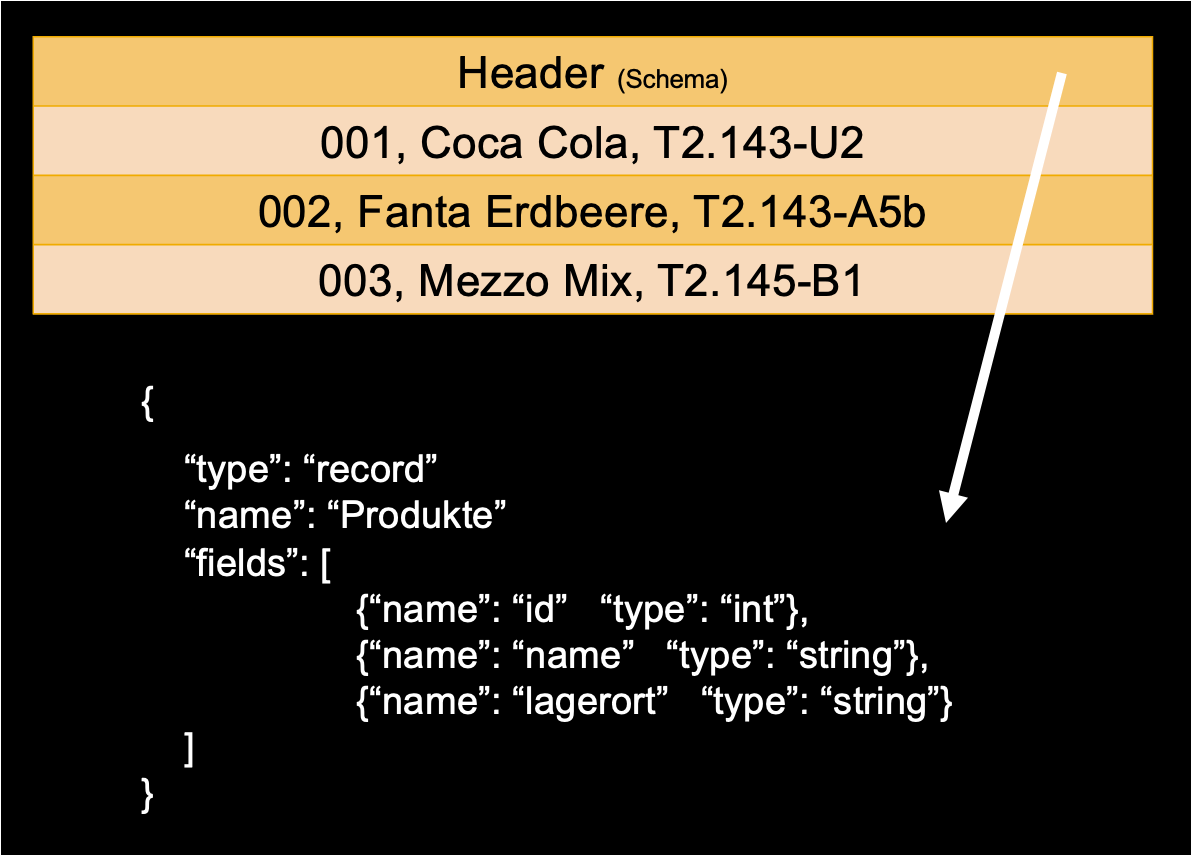
\includegraphics[width=1\textwidth]{Bilder/Avro.png} 
	\caption{Aufbau von Avro}
	\label{fig:Avro}
\end{figure}
\clearpage
\begin{figure}[ht]
	\centering
	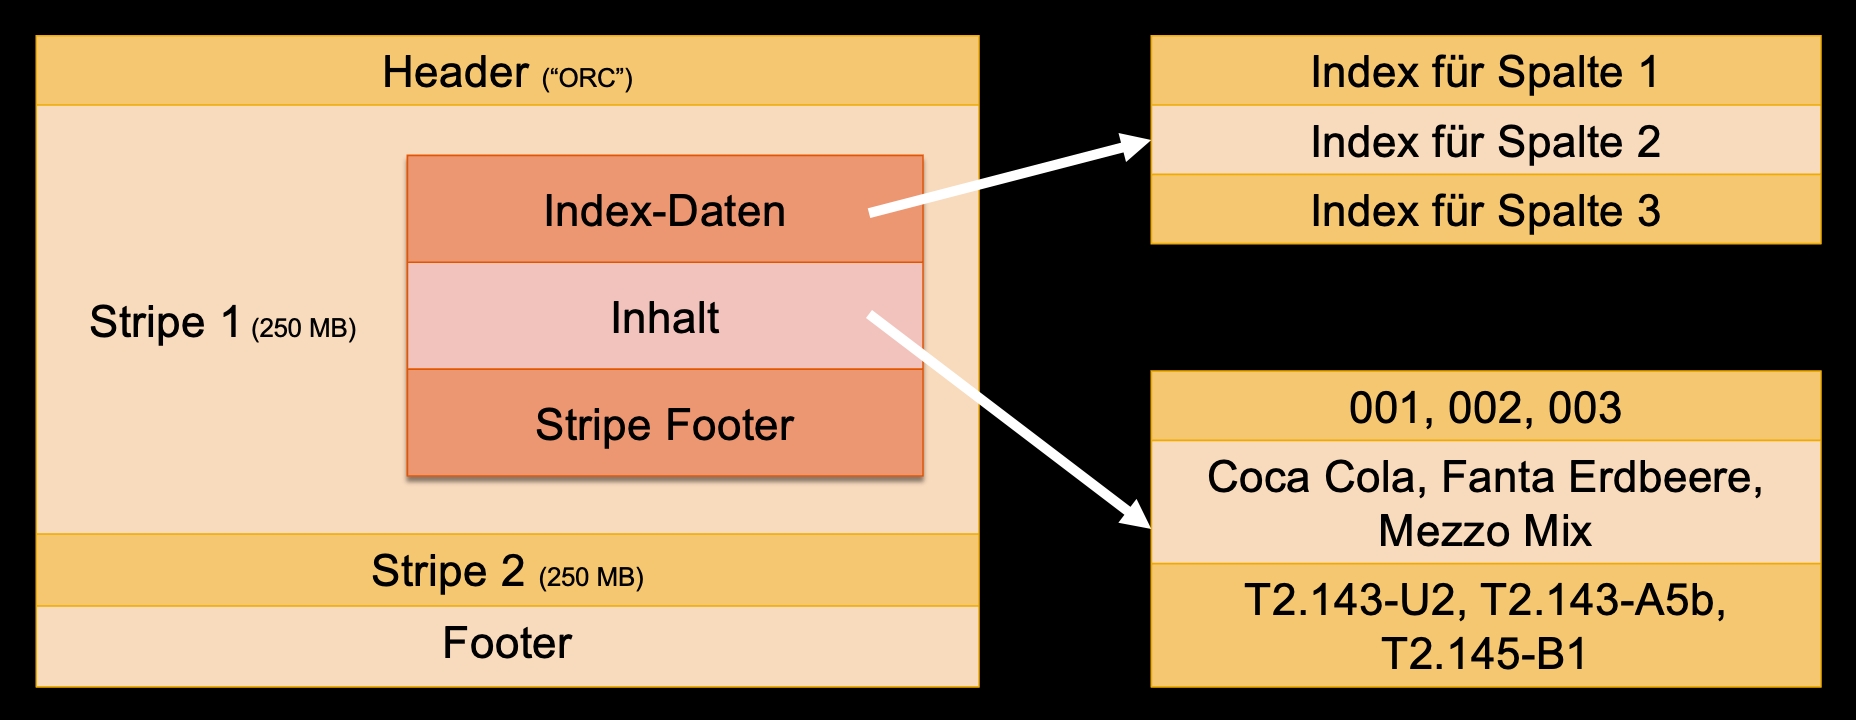
\includegraphics[width=1\textwidth]{Bilder/ORC.png} 
	\caption{Aufbau von ORC}
	\label{fig:ORC}
\end{figure}
\clearpage
\chapter{Vergleiche}
\begin{figure}[ht]
	\centering
	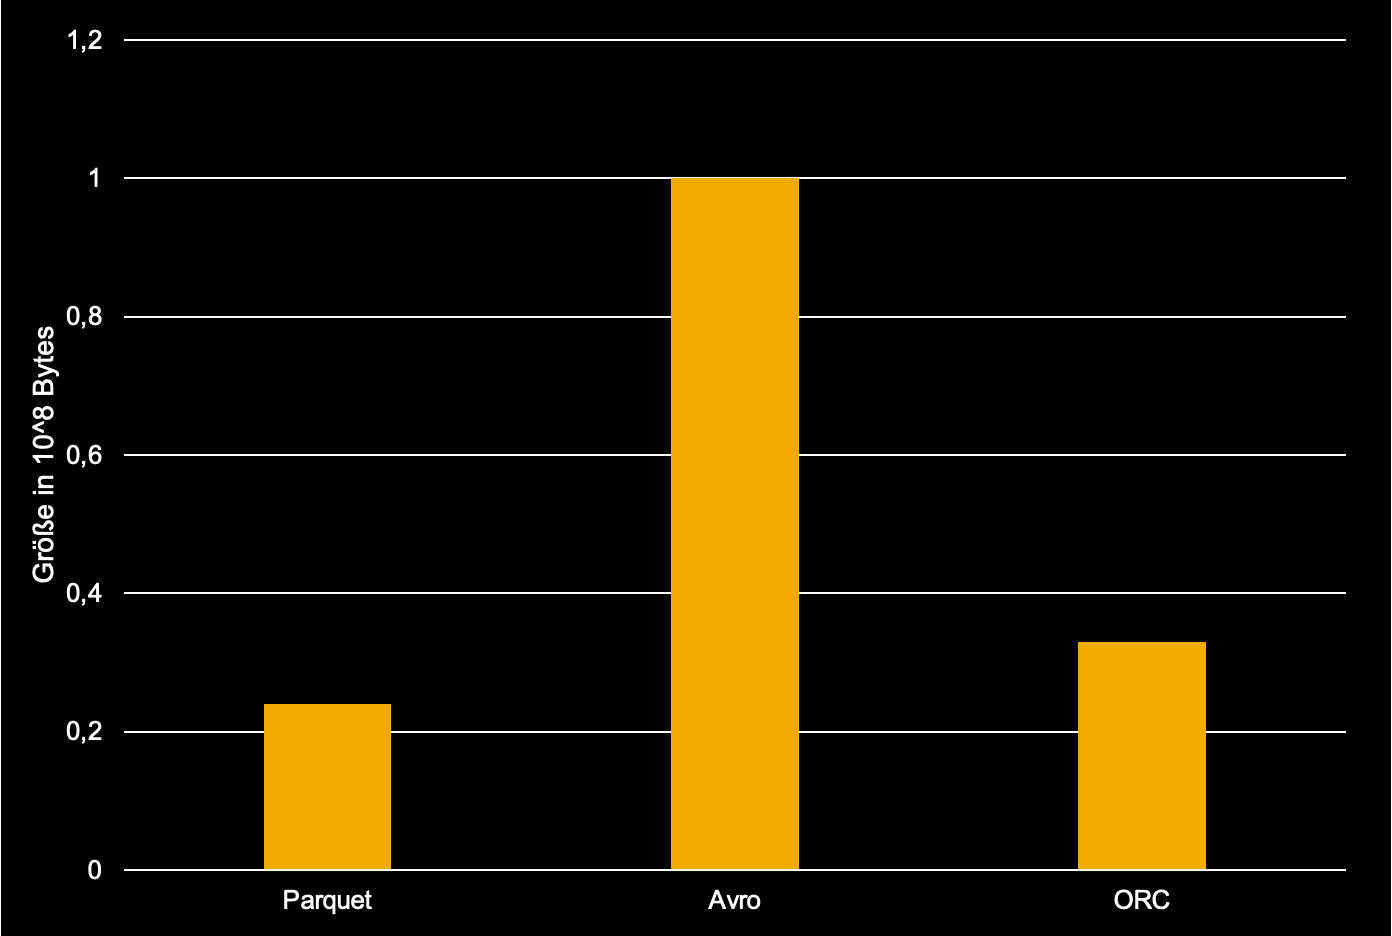
\includegraphics[width=1\textwidth]{Bilder/Speicher.png} 
	\caption{Speicherplatz}
	\label{fig:Speicherplatz}
\end{figure}
\clearpage
\begin{figure}[ht]
	\centering
	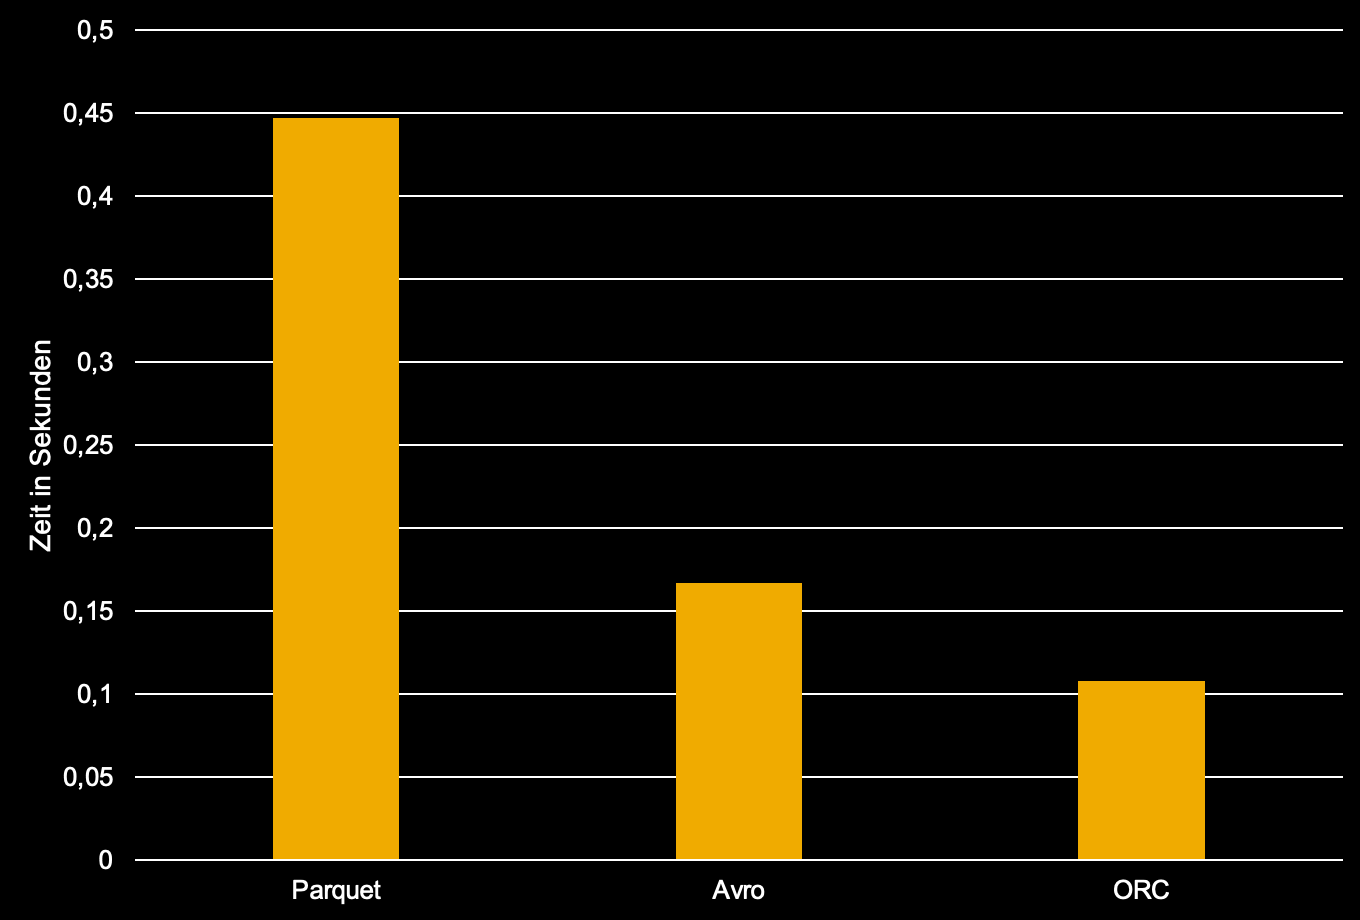
\includegraphics[width=1\textwidth]{Bilder/Lesezugriff.png} 
	\caption{Lesezugriff der gesamten Daten}
	\label{fig:Lesezugriff}
\end{figure}
\clearpage
\begin{figure}[ht]
	\centering
	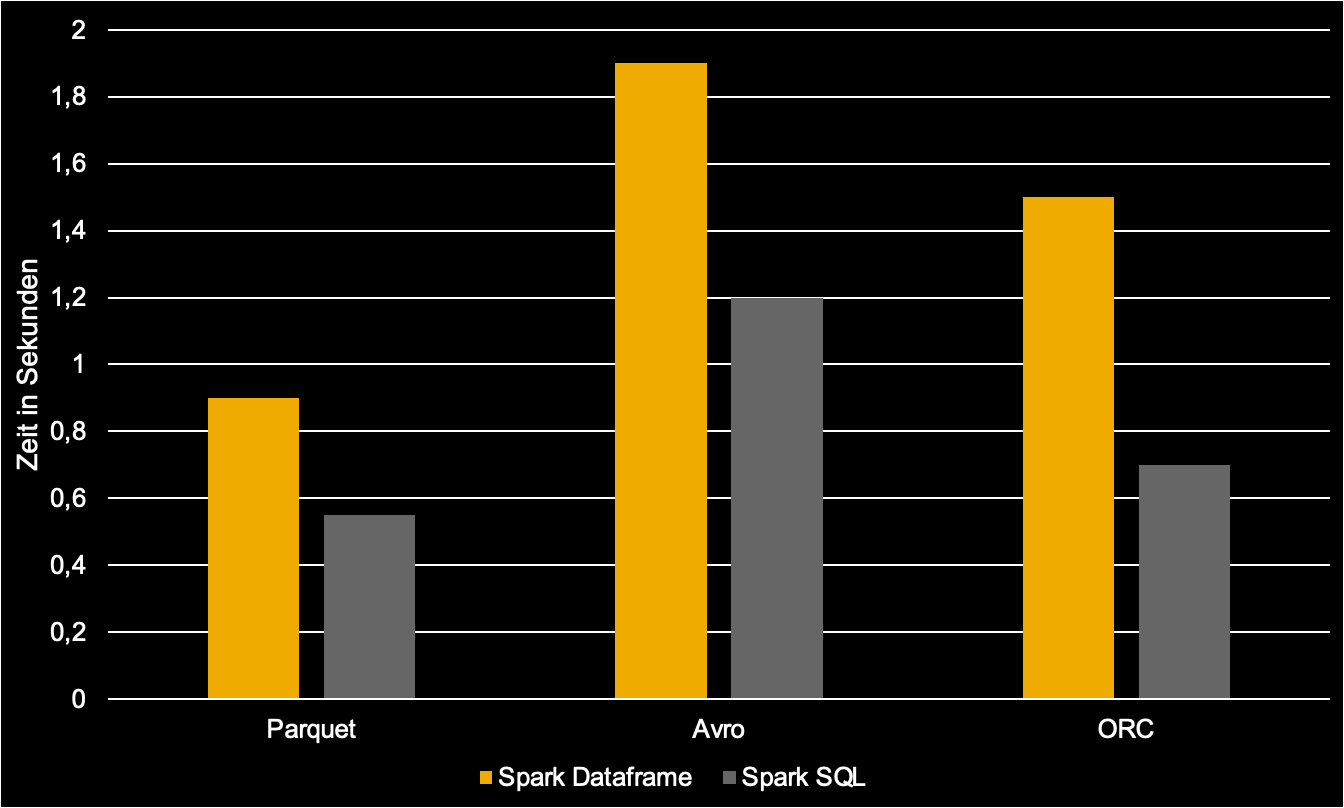
\includegraphics[width=1\textwidth]{Bilder/Zufall.png} 
	\caption{Zufällige Auswahl}
	\label{fig:Zufall}
\end{figure}
\clearpage
\begin{figure}[ht]
	\centering
	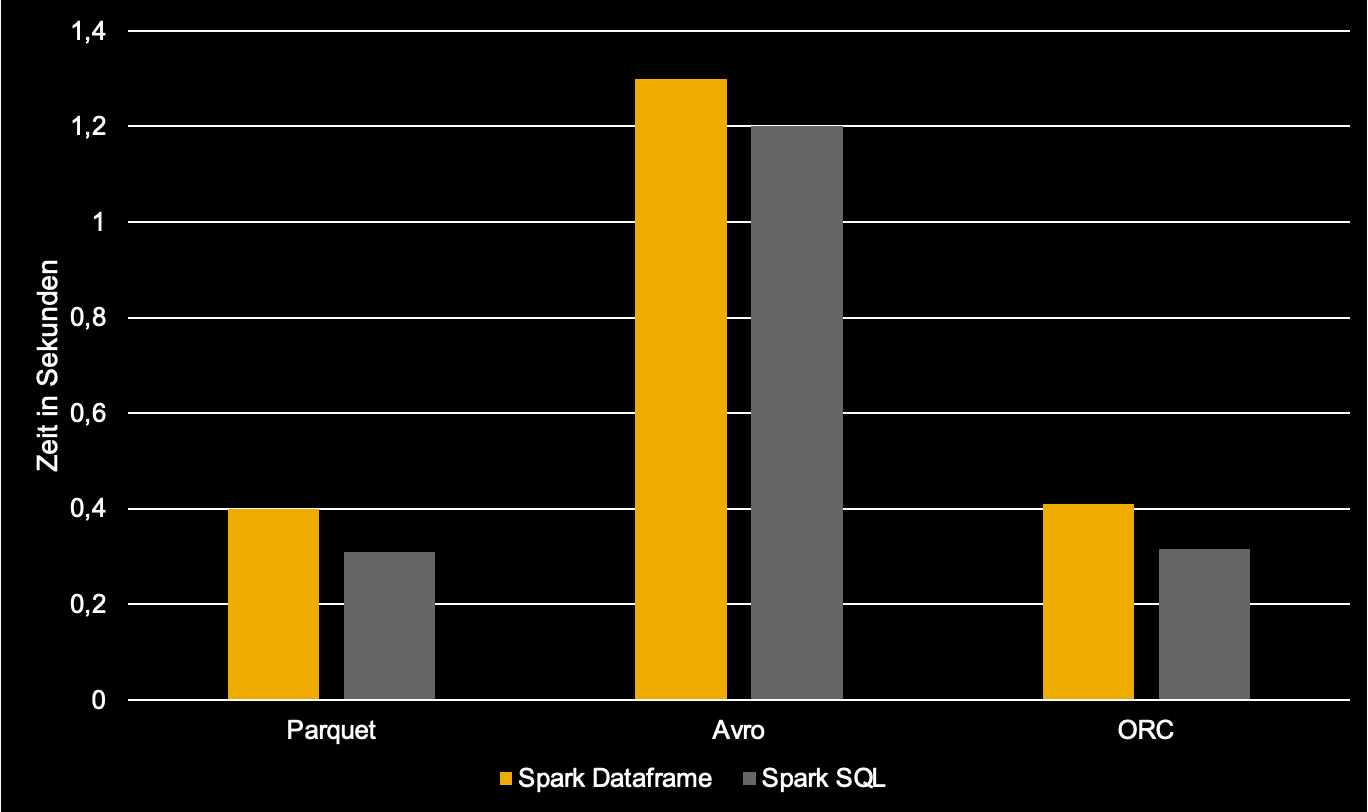
\includegraphics[width=1\textwidth]{Bilder/Aggregation.png} 
	\caption{Aggregation}
	\label{fig:Aggregation}
\end{figure}
\clearpage
\begin{figure}[ht]
	\centering
	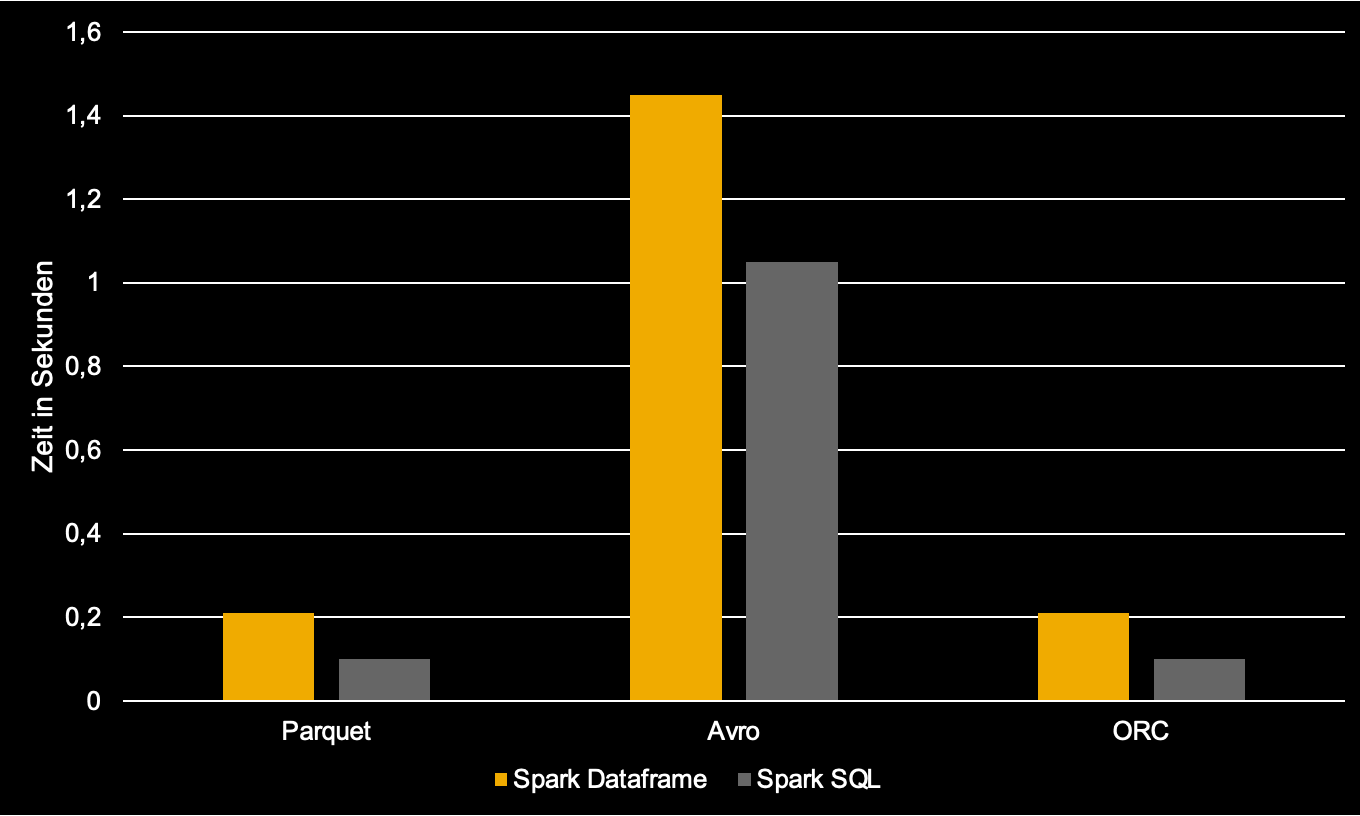
\includegraphics[width=1\textwidth]{Bilder/Summierung.png} 
	\caption{Summierung}
	\label{fig:Summierungen}
\end{figure}
\clearpage
\begin{figure}[ht]
	\centering
	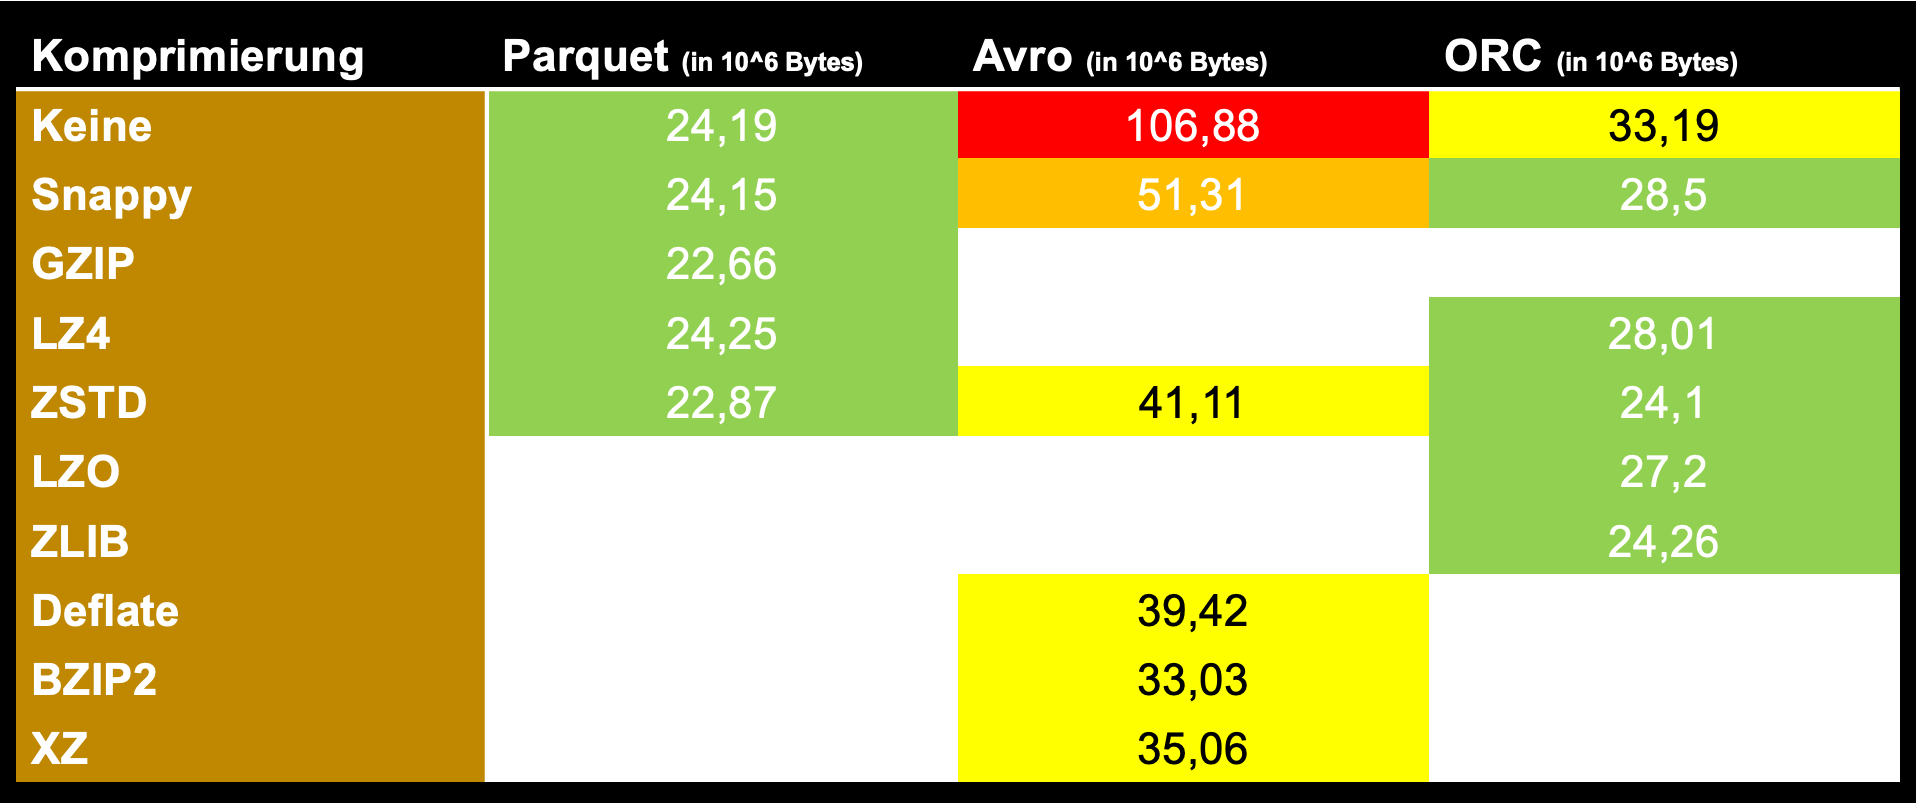
\includegraphics[width=1\textwidth]{Bilder/Komprimierung.png} 
	\caption{Komprimierung}
	\label{fig:Komprimierung}
\end{figure}
\clearpage
\chapter{Code}
\lstinputlisting[
    language=JavaScript,
	label=code:Parquet,    % Label; genutzt für Referenzen auf dieses Code-Beispiel
	caption=Parquet,
	captionpos=b,               % Position, an der die Caption angezeigt wird t(op) oder b(ottom)
	firstline=1,                % Zeilennummer im Dokument welche als erste angezeigt wird
	lastline=2              % Letzte Zeile welche ins LaTeX Dokument übernommen wird
]{Quellcode/code.js}
\lstinputlisting[
    language=JavaScript,
	label=code:Avro,    % Label; genutzt für Referenzen auf dieses Code-Beispiel
	caption=Avro,
	captionpos=b,               % Position, an der die Caption angezeigt wird t(op) oder b(ottom)
	firstline=4,                % Zeilennummer im Dokument welche als erste angezeigt wird
	lastline=9              % Letzte Zeile welche ins LaTeX Dokument übernommen wird
]{Quellcode/code.js}
\lstinputlisting[
    language=JavaScript,
	label=code:ORC,    % Label; genutzt für Referenzen auf dieses Code-Beispiel
	caption=ORC,
	captionpos=b,               % Position, an der die Caption angezeigt wird t(op) oder b(ottom)
	firstline=11,                % Zeilennummer im Dokument welche als erste angezeigt wird
	lastline=15              % Letzte Zeile welche ins LaTeX Dokument übernommen wird
]{Quellcode/code.js}
\lstinputlisting[
    language=JavaScript,
	label=code:XML,    % Label; genutzt für Referenzen auf dieses Code-Beispiel
	caption=XML,
	captionpos=b,               % Position, an der die Caption angezeigt wird t(op) oder b(ottom)
	firstline=41,                % Zeilennummer im Dokument welche als erste angezeigt wird
	lastline=55              % Letzte Zeile welche ins LaTeX Dokument übernommen wird
]{Quellcode/code.js}
\lstinputlisting[
    language=JavaScript,
	label=code:JSON,    % Label; genutzt für Referenzen auf dieses Code-Beispiel
	caption=JSON,
	captionpos=b,               % Position, an der die Caption angezeigt wird t(op) oder b(ottom)
	firstline=21,                % Zeilennummer im Dokument welche als erste angezeigt wird
	lastline=39              % Letzte Zeile welche ins LaTeX Dokument übernommen wird
]{Quellcode/code.js}
\lstinputlisting[
    language=JavaScript,
	label=code:CSV,    % Label; genutzt für Referenzen auf dieses Code-Beispiel
	caption=CSV,
	captionpos=b,               % Position, an der die Caption angezeigt wird t(op) oder b(ottom)
	firstline=17,                % Zeilennummer im Dokument welche als erste angezeigt wird
	lastline=19              % Letzte Zeile welche ins LaTeX Dokument übernommen wird
]{Quellcode/code.js}
\clearpage
\chapter{Datengrundlage}
\begin{figure}[ht]
	\centering
	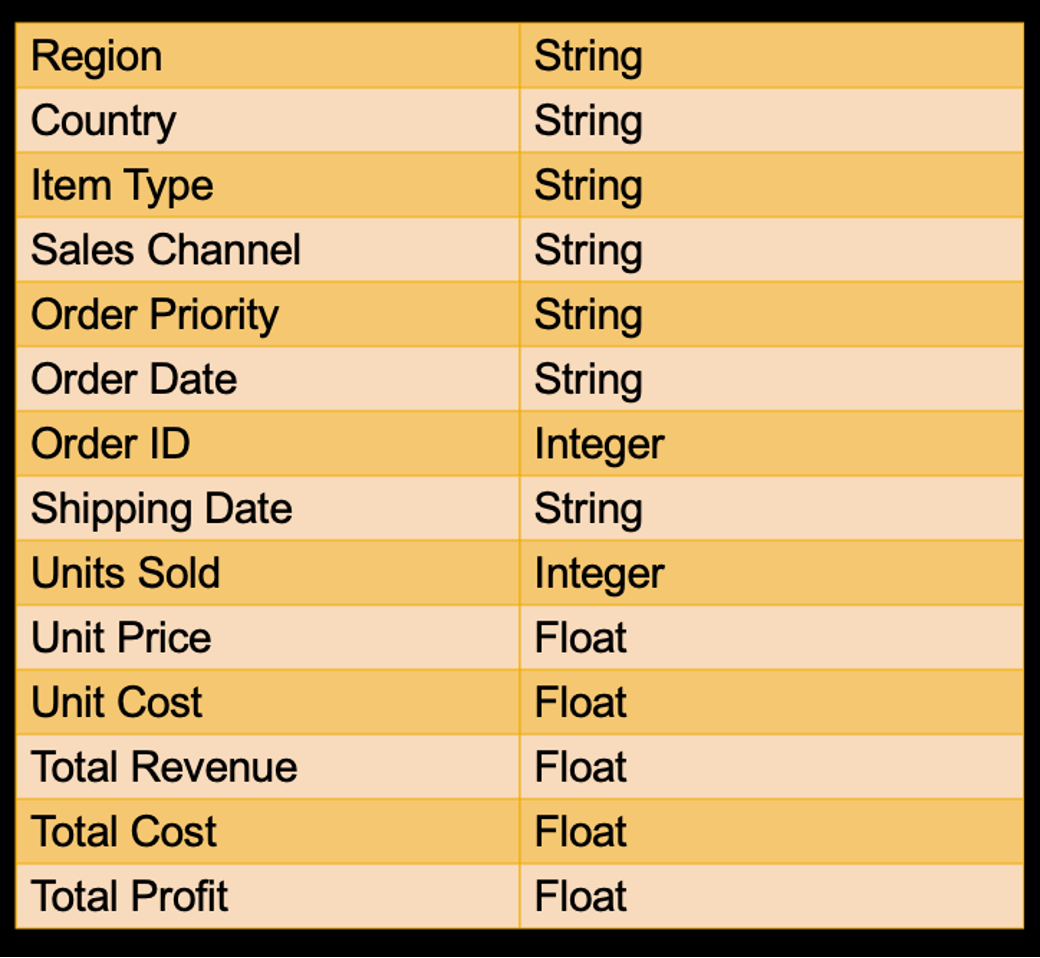
\includegraphics[width=1\textwidth]{Bilder/Daten.png} 
	\caption{Aufbau der Datengrundlage}
	\label{fig:Daten}
\end{figure}
